\documentclass[11pt,twoside,a4paper,cmspaper]{cms-tdr}
\usepackage{diagbox}
\def\svnVersion{aed52e2-D}\def\svnDate{2021/10/25}

\begin{document}\cmsNoteHeader{SMP-YY-XXX}

\newlength\cmsFigWidth
\newlength\cmsTabSkip\setlength{\cmsTabSkip}{1.7ex}
\ifthenelse{\boolean{cms@external}}{\setlength\cmsFigWidth{0.85\columnwidth}}{\setlength\cmsFigWidth{0.4\textwidth}}
\ifthenelse{\boolean{cms@external}}{\providecommand{\cmsTable}[1]{#1}}{\providecommand{\cmsTable}[1]{\resizebox{\textwidth}{!}{#1}}}
\newcommand{\mll}{m_{\ell\ell}}
\newcommand{\mjj}{m_\mathrm{jj}}
\newcommand{\mzg}{m_{\PZ\gamma}}
\newcommand{\etajj}{\abs{\Delta \eta_{\mathrm{jj}}}}
\newcommand{\gbarrel}{\gamma_{\text{barrel}}}
\newcommand{\gendcap}{\gamma_{\text{endcap}}}
\newcommand{\dphizgjj}{\Delta \phi_{\PZ\gamma,\mathrm{jj}}}
\newcommand{\mTH}{\ensuremath{\mT^{\PH}}\xspace}
\newcommand{\mTltwo}{\ensuremath{\mT^{l_{2}}}\xspace}
\newcommand{\ptvecll}{\ensuremath{\ptvec^{ll}}\xspace}
\newcommand{\ptll}{\ensuremath{\pt^{ll}}\xspace}
\newcommand{\dphill}{\ensuremath{\Delta\phi_{ll}}\xspace}
\newcommand{\drll}{\ensuremath{\Delta R_{ll}}\xspace}
\newcommand{\ptltwo}{\ensuremath{\pt^{l_{2}}}\xspace}
\newcommand{\ptvecltwo}{\ensuremath{\ptvec^{l_{2}}}\xspace}
\newcommand{\ttst}{\ensuremath{\ttbar\gamma{}+{}\PQt\PW}\xspace}
\newcommand{\tautau}{\ensuremath{\PGtp{}\PGtm}\xspace}

\cmsNoteHeader{SMP-22-006}
\title{Observation of $\PW\PW\gamma$ production and constraints on Higgs couplings to light quarks in proton-proton collisions at \texorpdfstring{$\sqrt{s}=13\TeV$}{sqrt(s) = 13 TeV}}

\author[cern]{The CMS Collaboration}

\date{\today}

\abstract{The first observation of the production of the triboson final state $\PW\PW\gamma$ in proton-proton collisions at a center-of-mass energy of 13\TeV is presented. A data set corresponding to an integrated luminosity of 138\fbinv, collected by the CMS experiment at the LHC in 2016--2018 is used. Events are selected by requiring exactly two leptons (one electron and one muon) of the opposite charge, moderate missing transverse momentum, and a photon. The measured fiducial cross section for $\PW\PW\gamma$ is $\sigma=XXX\unit{fb}$, in good agreement with the next-to-leading order QCD prediction. Exclusion limits on anomalous quartic gauge couplings are derived at 95\% confidence level in terms of the dimension-8 effective field theory operators. The analysis is also extended to search for Higgs photon associated production where the Higgs decays into $\PW\PW$, which is sensitive to the Higgs coupling with light quarks, \PQc, \PQs, \PQu and \PQd, and a set of limits on these couplings are reported at 95\% confidence level.}

\hypersetup{
pdfauthor={Ying An, Zhe guan, Andrew Michael Levin, Qiang Li, Meng Lu, Sen Deng, Jie Xiao, Sitian Qian, Jing Peng, Congqiao Li, Qilong Guo},
pdftitle={Measurement of the triboson WWgamma production in proton-proton collisions at sqrt(s) = 13 TeV and constraints of couplings on anomalous quartic gauge and Higgs to the light quarks},
pdfsubject={CMS},
pdfkeywords={CMS,  multi-boson, Yukawa couplings}}

\maketitle 

Multi-boson and specifically tri-boson productions are among the forefronts of testing the standard model (SM), and became only accessible at the LHC thanks to its high collision energy and large luminosity of data collected. Previously, three massive gauge boson (\PV\PV\PV with \PV = \PW, \PZ) productions have been observed by the CMS and ATLAS experiments, respectively~\cite{CMS:2020hjs,ATLAS:2021atz}. The non-abelian nature of the electroweak interaction predicts the presence of self-interacting vector boson vertices. The $\PW\Pgg\Pgg$ and $\PZ\Pgg\Pgg$ productions have been measured by the ATLAS and CMS experiments, with corresponding signal significance reaching or above 3 and 5 standard deviations~\cite{ATLAS:2015ify,ATLAS:2016qjc,CMS:2017tzy,CMS:2021jji}, respectively. In this letter, we are interested in another type of tri-boson production process, i.e. $\PW\PW\gamma$ production. The related measurements have been performed at the CMS and ATLAS experiment, at a center-of-mass energy of 8\TeV~\cite{CMS:2014cdf,ATLAS:2017bon}. The upper limit on the production cross sections are reported therein, due to lack of statistics and sensitivity.

Tri-boson productions can be sensitive to the values of triple and quartic gauge couplings (TGCs and QGCs). The measurement of possible deviations from the theoretical predictions could provide indirect evidence of new particles or new interactions. The same final states can also be exploited to probe Higgs couplings with light quarks, \PQc, \PQs, \PQu and \PQd, as proposed in recent literature~\cite{Khanpour:2017inb,Aguilar-Saavedra:2020rgo,Falkowski:2020znk}. As the leading order (LO) gluon-initiated contribution $gg\rightarrow h\gamma$ vanishes due to Furry’s theorem, the inclusive $h\gamma$ production at the LHC is directly related to Higgs Yukawa coupling with the light quarks. Recently, ATLAS provides a bound on the charm Yukawa coupling modifier $\kappa_c<8.5$ at the 95\% confidence level~\cite{ATLAS:2021zwx}, while the upper bound on the strange Yukawa coupling is quite loose~\cite{Duarte-Campderros:2018ouv,ATLAS:2018xfc}.

At leading order in quantum chromodynamics (QCD), $\Pe^+\nu_{\Pe}\mu^-\overline{\nu}_{\mu}\Pgg$ and $\mu^+\nu_{\mu}\Pe^-\overline{\nu}_{\Pe}\Pgg$ production in $\Pp\Pp$ collisions can proceed through photons' initial-state radiation (ISR) from one of the incoming quarks, final-state radiation (FSR) from the outgoing charged leptons, the $\PW\PW\Pgg$ TGC, $\PW\PW\PZ\Pgg$ or $\PW\PW\Pgg\Pgg$ QGC vertices. Example diagrams are shown in Fig.~\ref{fig:LO diagrams}. At higher orders in QCD~\cite{Zhu:2020ous}, additional quarks can appear in the final state, and the photon can arise by FSR from an outgoing quark or lepton. 

\begin{figure*}[htp]
    \centering
    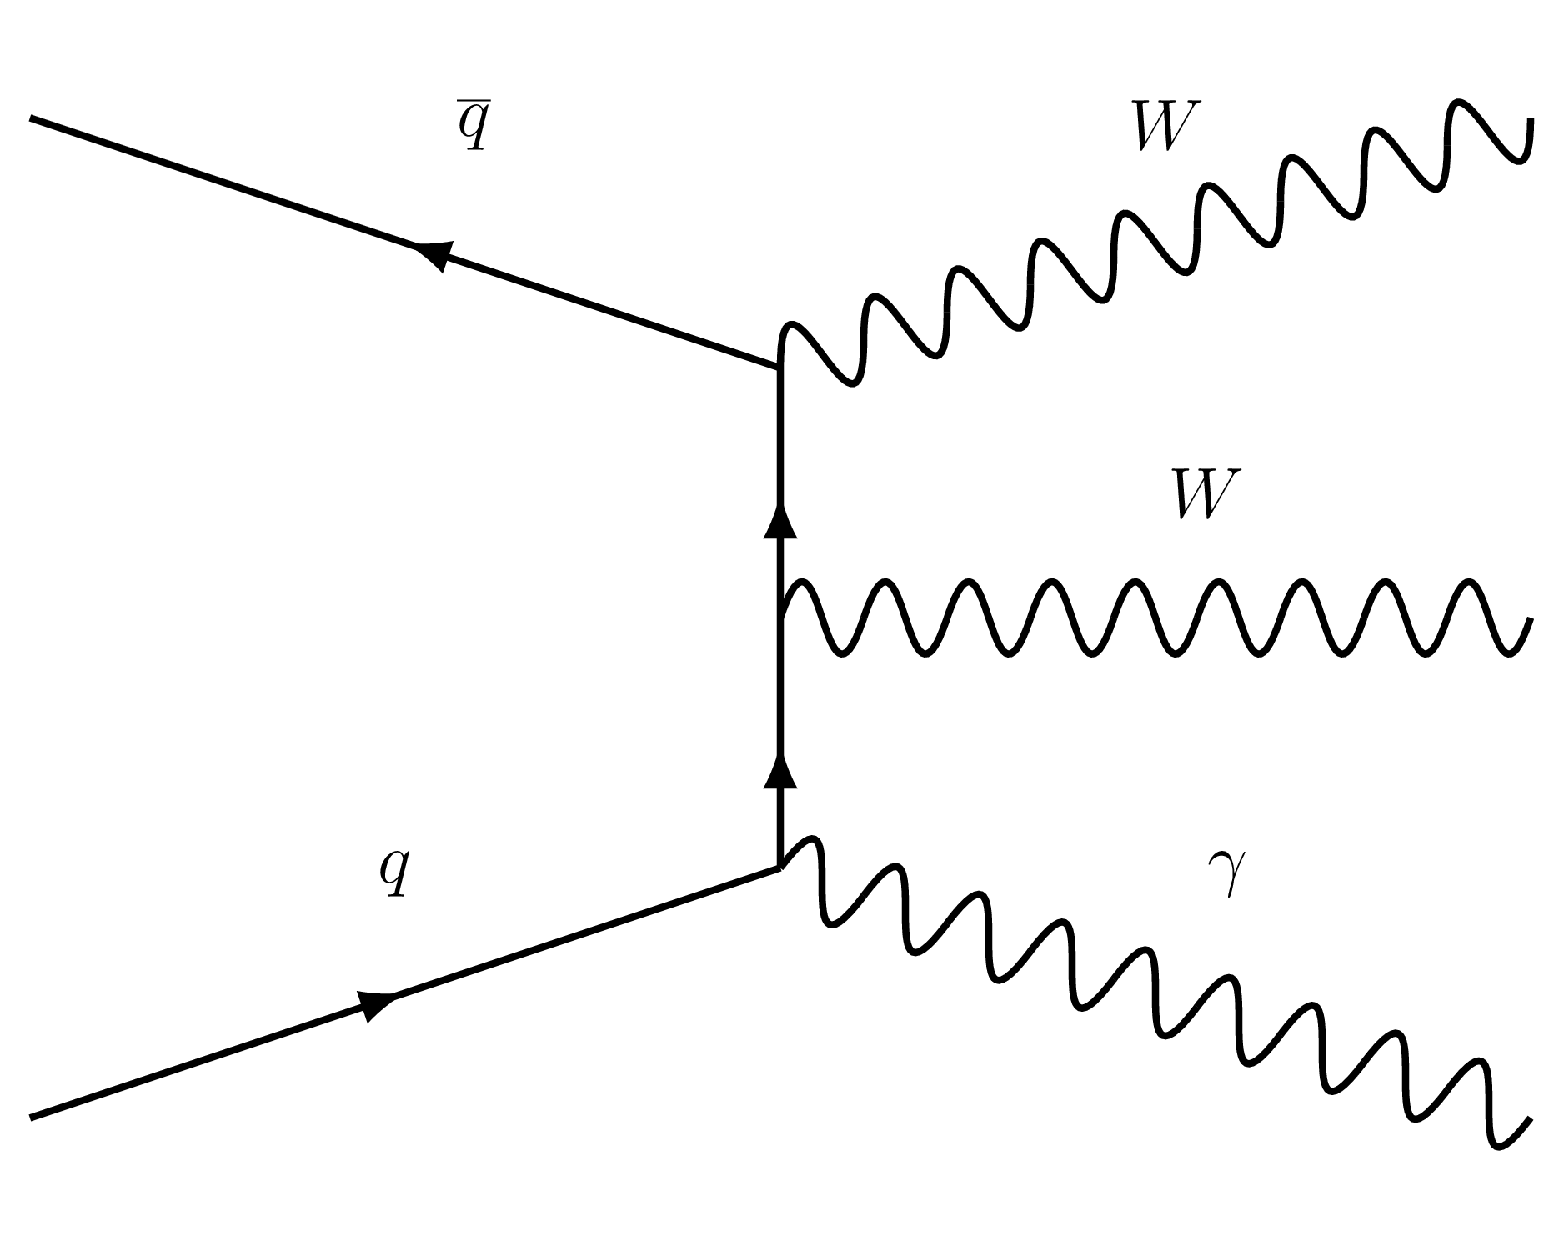
\includegraphics[width=0.22\textwidth]{ISR.pdf}
    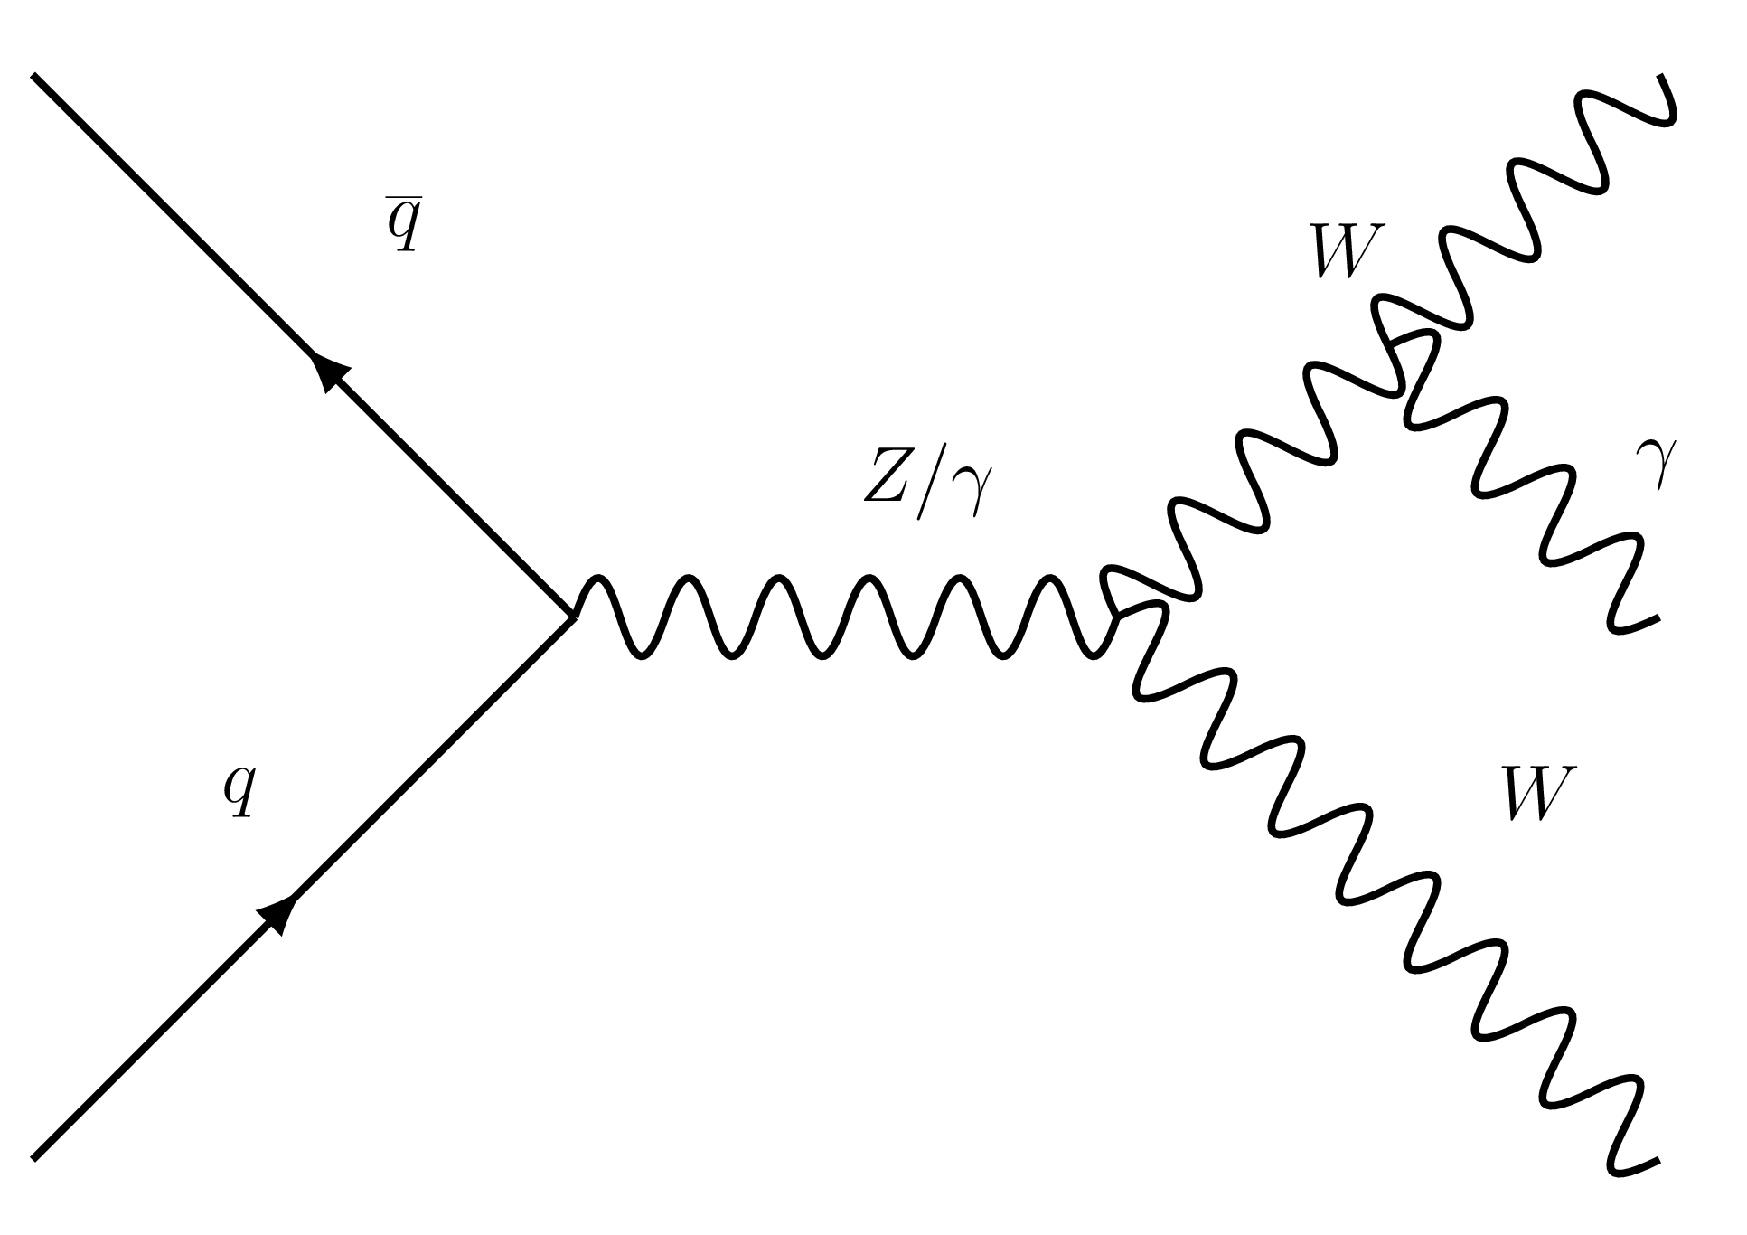
\includegraphics[width=0.22\textwidth]{FSR.pdf}
    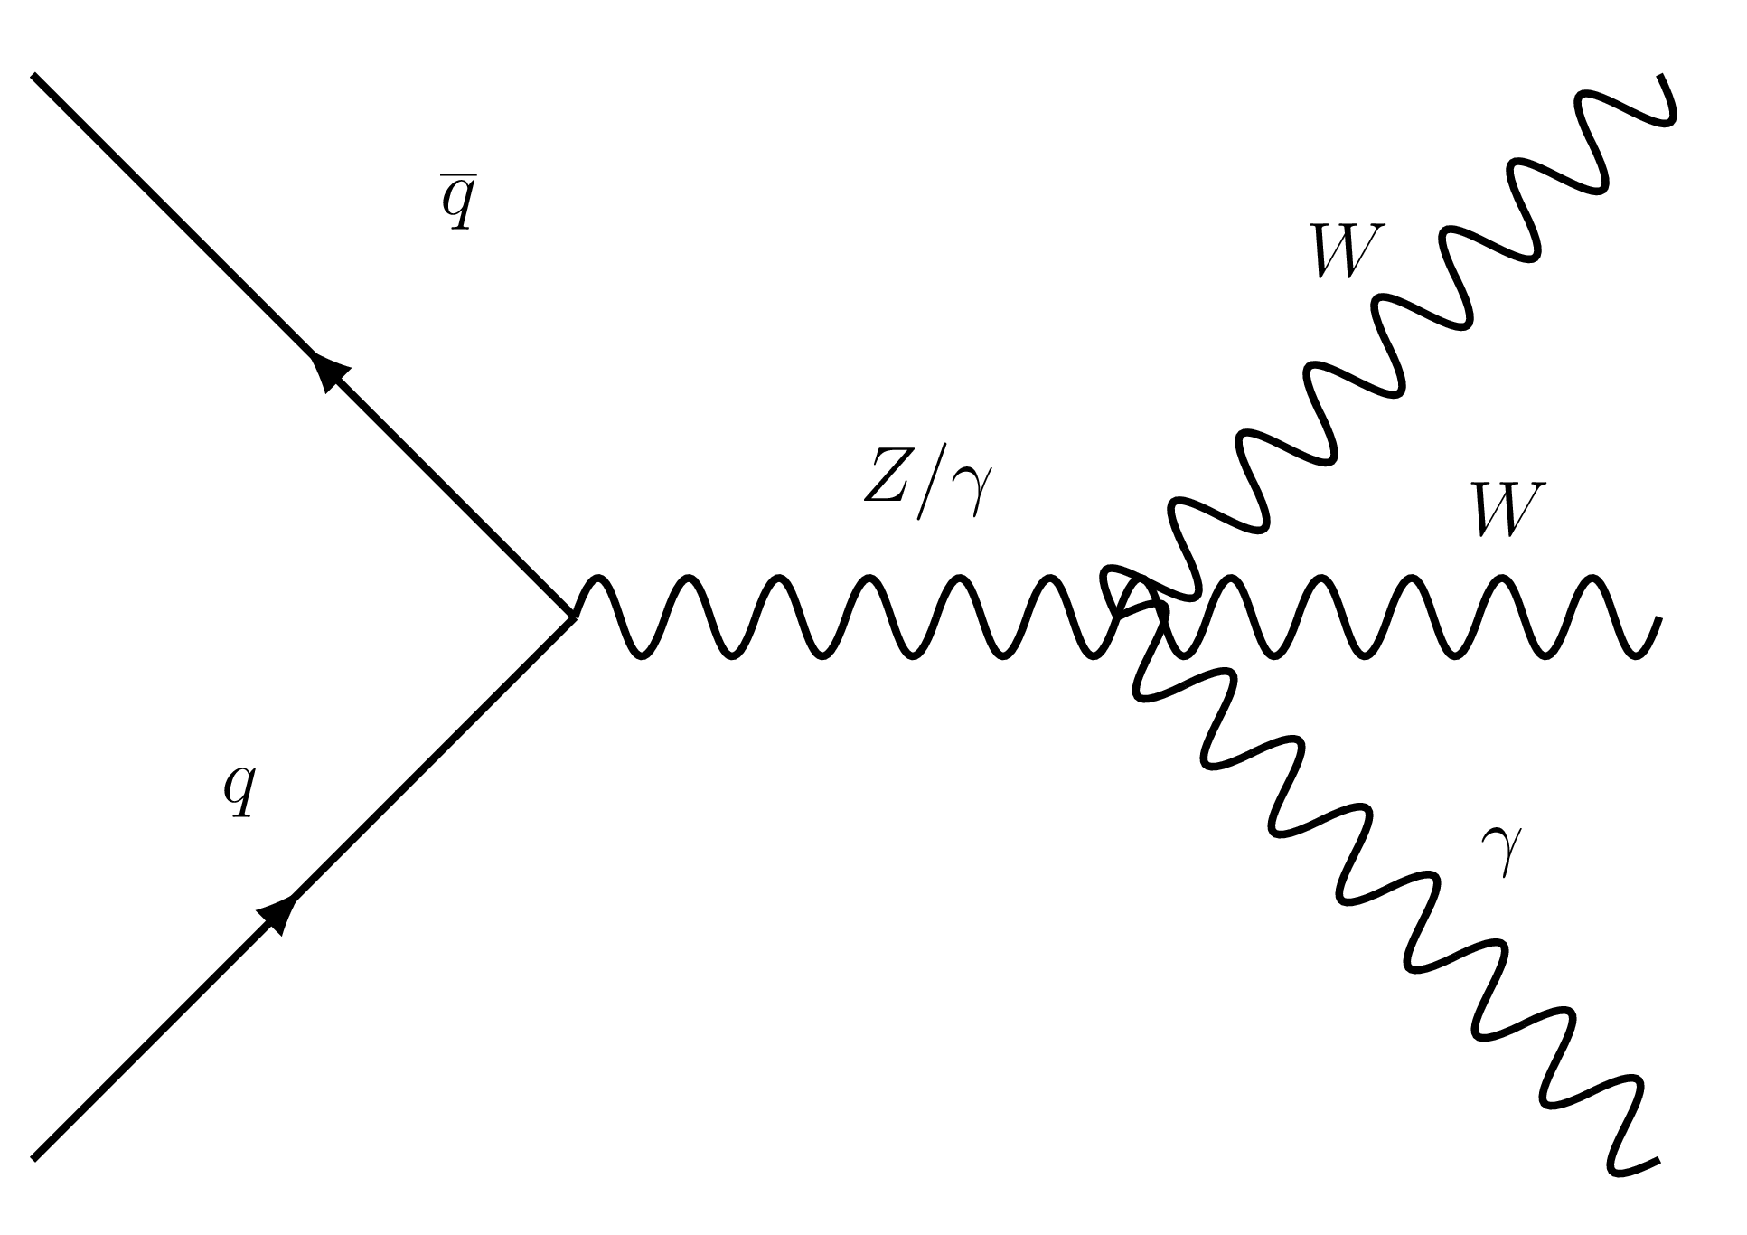
\includegraphics[width=0.22\textwidth]{aQGC.pdf}
    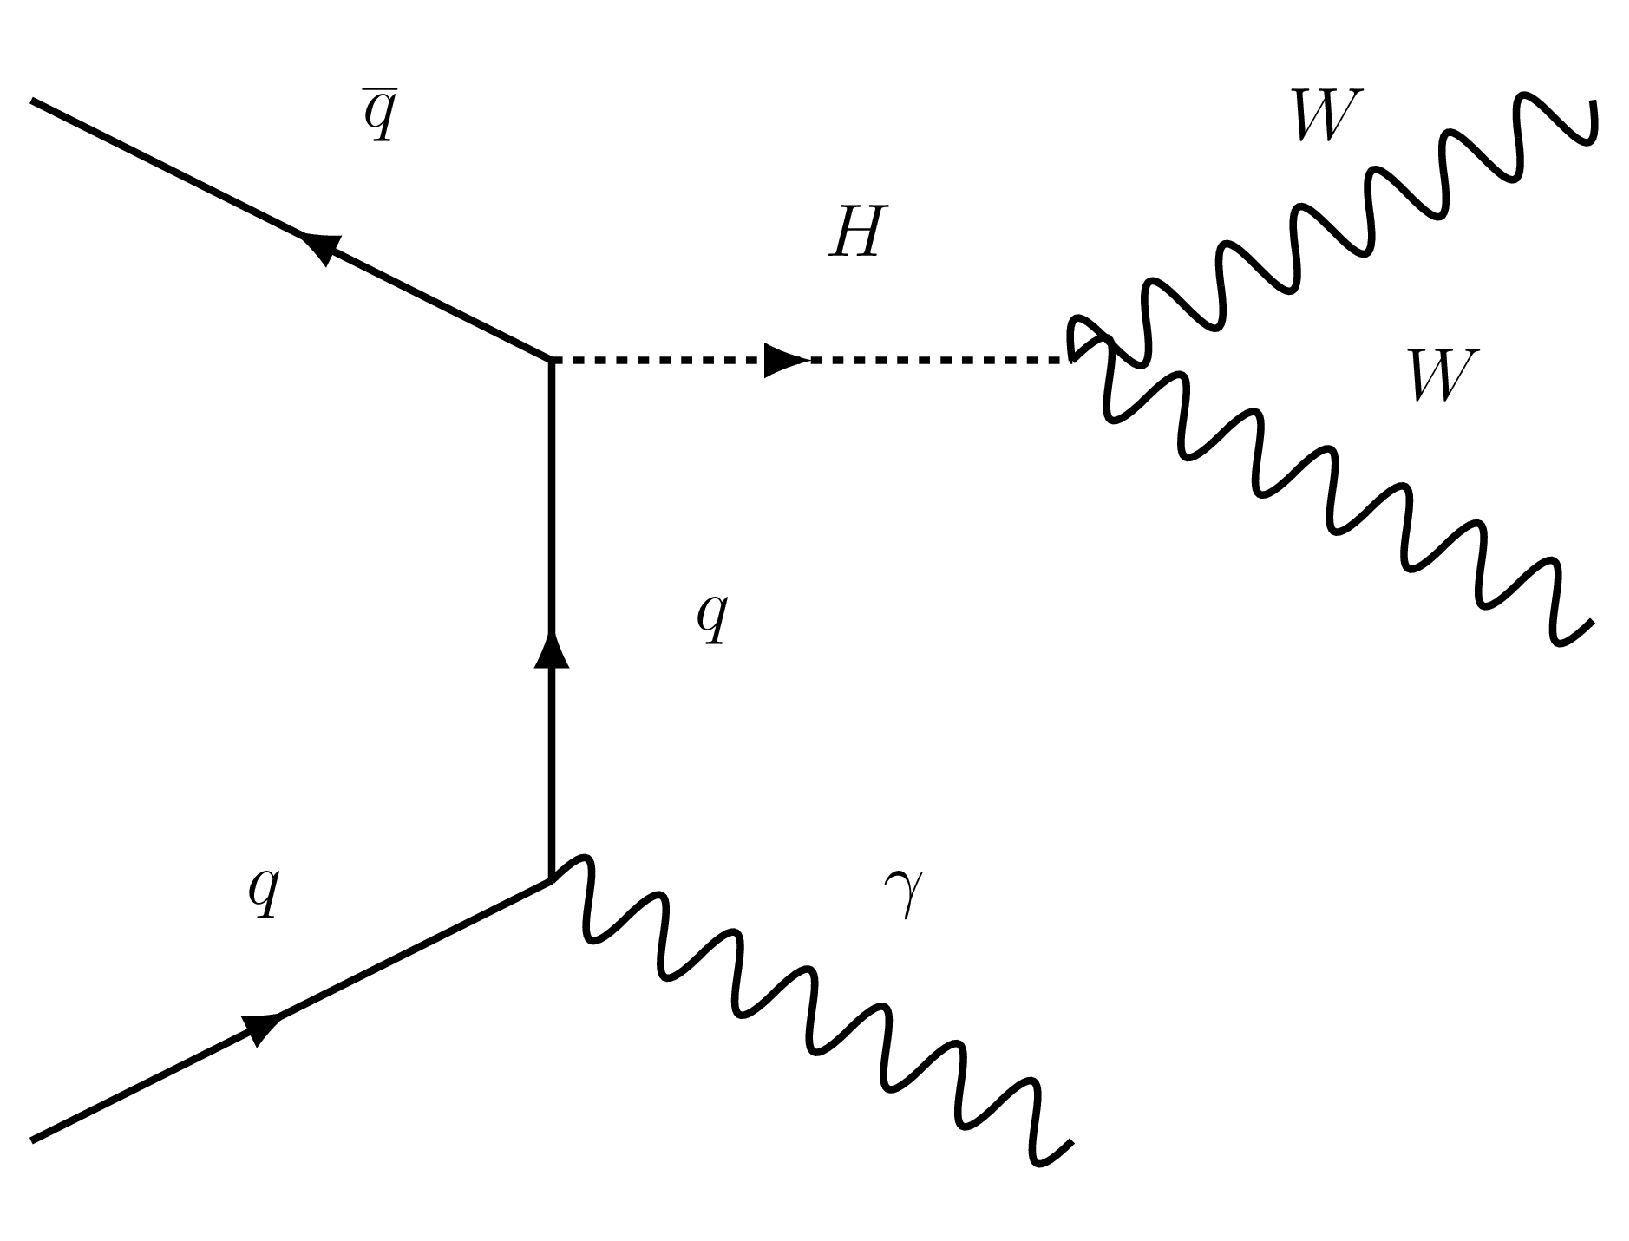
\includegraphics[width=0.22\textwidth]{HG.pdf}
    \caption{Representative Feynman diagrams for $\PW\PW\gamma$ process: ISR, FSR, QGC, and Higgs associated productions, from the left to right.}
    \label{fig:LO diagrams}
\end{figure*}

This letter reports the first observation of the triboson $\PW\PW\gamma$ production in proton-proton collisions, together with the probe of Higgs couplings with light quarks, based on proton-proton collision data at $\sqrt{s} = 13\TeV$ collected by the CMS experiment at the CERN LHC during 2016--2018, corresponding to an integrated luminosity of $138\fbinv$.

The central feature of the CMS apparatus is a superconducting solenoid of 6\unit{m} internal diameter, providing a magnetic field of 3.8\unit{T}. Within the solenoid volume, there are a silicon pixel, a strip tracker, a lead tungstate crystal electromagnetic calorimeter, and a brass and scintillator hadron calorimeter, each composed of a barrel and two endcap sections. Forward calorimeters extend the pseudorapidity ($\eta$) coverage provided by the barrel and endcap detectors. Muons are detected in gas-ionization chambers embedded in the steel flux-return yoke outside the solenoid. A detailed description of the CMS detector, together with a definition of the coordinate system used and the relevant kinematic variables, can be found in Ref.~\cite{Chatrchyan:2008zzk}.

Electrons and photons are measured in the range $\abs{\eta} < 2.5$ defined by the tracker acceptance. The energy of electrons is a combination of three measurements: the electron momentum at the primary interaction vertex as determined by the tracker~\cite{pvdefinition}, the energy of the corresponding ECAL cluster, and the energy sum of all bremsstrahlung photons spatially compatible with originating from the electron track. The photon momentum is determined solely using the energy measurement in the ECAL. The photon's ECAL cluster is required to be inconsistent with a charged-particle track reconstructed in the tracker~\cite{cmscollaboration2020electron}. Muons are measured in the pseudorapidity range $\abs{\eta} < 2.4$ and their momenta are determined using a global fit of muon measurements in the gas-ionization chambers and matched tracks in the silicon tracker~\cite{Sirunyan:2018}.

The missing transverse momentum vector $\ptvecmiss$ is computed as the negative vector \pt sum of all measured particles in an event, reconstructed with the particle flow algorithm~\cite{CMS-PRF-14-001}, and its magnitude is denoted by $\ptmiss$~\cite{Sirunyan_2019}. The $\ptvecmiss$ of an event is intended to represent the neutrinos associated with a single $\Pp \Pp$ interaction within a bunch crossing. The contribution to $\ptvecmiss$ due to particles from additional $\Pp \Pp$ interactions within the same bunch crossing (pileup) is mitigated through the pileup-per-particle identification algorithm~\cite{Bertolini:2014bba,cmspuppi}. The $\ptvecmiss$ is also modified to include corrections to the energy scale and resolution of the reconstructed jets in the event.

The signal is simulated at next-to-leading order (NLO) using with the \MGvATNLO 2.6.5 generator~\cite{MGatNLO}. The parton showering and hadronization are performed using {\PYTHIA}8 version 8.226~\cite{Sjostrand:2014zea}, and the detector simulation is performed using \GEANTfour~\cite{AGOSTINELLI2003250}. To match data-taking conditions, we generate three sets of events corresponding to $2016$, $2017$, and $2018$. The {\PYTHIA}8 CUETP8M1~\cite{Khachatryan:2015pea} tune with the NNPDF30\_nlo\_nf\_5\_pdfas~\cite{Ball_2015} parton distribution functions (PDFs) are used for the $2016$ simulation, and the {\PYTHIA}8 CP5~\cite{Sirunyan:2019dfx} tune with the NNPDF31\_nnlo\_hessian\_pdfas~\cite{collaboration2017parton} PDFs are used for the $2017$ and $2018$ simulations. The simulations include $\PW \to \Pgt \Pgngt$ decays, which are considered part of the signal when a $\Pgt$ decays with an emission of an electron or a muon. No EW or NNLO QCD corrections are applied.

We select $\PW^+\PW^-\Pgg\to$ $\Pe^+\nu_{\Pe}\mu^-\overline{\nu}_{\mu}\Pgg$ and $\mu^+\nu_{\mu}\Pe^-\overline{\nu}_{\Pe}\Pgg$ events from the set of events that pass a level-one~\cite{Sirunyan:2020zal} and a set of  high-level~\cite{Khachatryan:2016bia} triggers that most of them require a muon together with an electron that are both isolated from other detector activity and, therefore, are likely to be promptly produced as opposed to produced during the hadronization of a jet. \iffalse To increase statistics, a combination of datasets are used and The $\pt$ thresholds of the high-level trigger leading and trailing leptons are $25$ and $15\GeV$, respectively.\fi We require the presence of a single high-quality~\cite{CMS:EGM-14-001} reconstructed photon, $\ptmiss$ exceeding $20\GeV$, and that the isolated electron or muon satisfies additional quality criteria~\cite{Sirunyan:2018,Khachatryan:2015hwa}. Offline kinematical requirements on the selected objects, based on the detector acceptance and the trigger thresholds, are photon $\pt > 20\GeV$, photon $\abs{\eta} < 2.5$, electron (muon) $\abs{\eta}< 2.5$ (2.4), leading (sub-leading) lepton $\pt > $ 25 (15) \GeV. To reduce the background from $\PW\PZ\Pgg$ events, we reject events that contain an additional muon or electron with $\pt > 10\GeV$ that satisfies minimal quality criteria. Moreover, $\Delta R = \sqrt{\smash[b]{\left(\Delta\eta\right)^2 + \left(\Delta\phi\right)^2}}$, where $\Delta \phi$ and $\Delta \eta$ are the spatial separations in azimuthal angle $\phi$ (in radians) and $\eta$ between the lepton and photon, is required to exceed $0.5$. We further optimize signal and suppress backgrounds, requiring the dilepton mass ($\mll$) and transverse momentum ($\ptll$) to be larger than 20 and 30 GeV, respectively, the transverse mass of the Higgs boson, $\mTH = \sqrt{2 \ptll \ptmiss \left[1 - \cos\Delta\phi(\ptvecll, \ptvecmiss)\right]}$ to be larger than 50 GeV. \iffalse and the trailing lepton's transverse mass $\mTltwo = \sqrt{2 \ptltwo \ptmiss \left[1 - \cos\Delta\phi(\ptvecltwo, \ptvecmiss)\right]}$, larger than 20 GeV. \fi  Finally, for the Higgs searches, we require $\dphill<2.5$ and $\drll<2.3$, as the two oppositely charged W bosons from Higgs decay tends to have opposite spin orientation and the leptons from W bosons are likely to travel in the same direction~\cite{Dittmar:1996ss}, and considering the two oppositely charged W bosons are off-shell in this case, a looser cut for $\mTH > 40\GeV$ is used.

Background processes containing a prompt lepton and a prompt photon, including $\PZ\Pgg$ production, $\ttbar\Pgg$ production and single top production are simulated using \MGvATNLO and {\PYTHIA}8, in a manner similar to that for the signal samples. The background due to events containing nonprompt leptons and photons, including those from instrumental mismeasurements and genuine leptons or photons within jets, is estimated from data similar as done in Ref.~\cite{CMS:2021foa}. The ratio of well-isolated, high-quality leptons to less-well-isolated, lower-quality leptons is measured in a dijet control region in data as a function of the lepton $\abs{\eta}$ and $\pt$, and corrected for prompt leptons and prompt photon conversions based on simulated samples. A similar procedure is applied for photons based on a $\PW$+jets control region that excludes the signal region. In the nonprompt photon case, a fit to the width of the photon ECAL shower is used to determine the nonprompt photon fraction in the well-isolated, high-quality category, as described in Ref.~\cite{Sirunyan_2020}. The two procedures are combined in a way that avoids double counting to estimate the contribution from events containing both a nonprompt lepton and a nonprompt photon. 

\iffalse A control region enriched with same charge W boson pairs is used to validate nonprompt lepton backgrounds, by requiring electron and muon charge to be the same together with $\mTH<60$\,GeV on top of the signal selections . Furthermore,\fi A control regions enriched with {\ttst} is used to validate nonprompt lepton backgrounds first and then it will be used to constrain the estimates of these processes in the simultaneous fit. The definition of {\ttst} control region follow that of the signal region closely to make the event kinematics similar. Specifically, the control region share all event selection criteria with the signal region except for the requirements on \iffalse $\mll$, $\mTH$, $\mTltwo$, and the number of {\cPqb}-tagged jets. The {\ttst} control region instead requires $\mll > 50\GeV$  and \fi at least one {\cPqb}-tagged jet with $\pt > 20\GeV$. \iffalse If there is another jet in the event with $\pt > 30\GeV$, the {\cPqb}-tagged jets must also have $\pt > 30\GeV$. There is no constraint on {\mTH}, and the requirement $\mTltwo > 30\GeV$ is common with the signal region. The {\tautau} control region requires $40 < \mll < 80\GeV$ and $\mTH < 60\GeV$, and has no constraint on $\mTltwo$. The restriction of having no {\cPqb}-tagged jets with $\pt > 20\GeV$ is common with the
signal region. \fi

The observed distributions of photon \pt and $\mTH$ are compared with the expected distributions based on the \MGvATNLO simulation in Fig.XXX. The experimental data agrees with the prediction within uncertainties. The expected and observed numbers of events are listed in Table.YYY.

A variety of sources of systematic uncertainty are considered as nuisance parameters in the fit subject to log-normal constraints. Experimental sources of systematic uncertainty include: the jet energy scale and resolution (which affect the $\ptvecmiss$), the lepton and photon identification efficiencies, the pileup modeling, the integrated luminosity measurement, the statistical power of our simulated samples and data control regions, and the nonprompt photon and nonprompt lepton background estimation methods. Theoretical sources of systematic uncertainty include: the renormalization and factorization QCD scales, and PDFs. The renormalization and factorization QCD scales are varied by factors of $2$ and $1/2$, excluding the (2,1/2) and (1/2,2) cases, and the envelope of these variations is taken as the uncertainty. The systematic uncertainty due to the PDFs is calculated using the 32 additional members of the PDF4LHC15\_nnlo\_30\_pdfas PDF set following the PDF4LHC prescription for a Hessian PDF set~\cite{Butterworth_2016,Harland_Lang_2015,Ball_2015,PhysRevD.93.033006}. The uncertainties in the photon identification efficiency ($1$--$4$\%, depending on the photon \pt and $\eta$) and the integrated luminosity measurement (1.8\%) have the largest impact on the measurement.

The signal strength is extracted from a binned maximum likelihood fit to the photon \pt and $\mTH$ distributions, where the likelihood function is the product of a Poisson probability density function for each bin. A simultaneous fit in both signal and control regions is used for our results. The theoretical predictions of the cross section are $XXX \pm XXX \text{ (scale)} \pm XXX \text{ (PDF)} \unit{pb}$ based on the NLO QCD \MGvATNLO simulation. The measured cross section from the simultaneous fit with the uncertainties divided into statistical, experimental, and theoretical components is $\sigma = XXX \pm XXX \unit{pb} =XXX \pm XXX \stat \pm XXX \syst \pm XXX \thy \unit{pb}$. 

Next, we search for \iffalse anomalous quartic gauge couplings (aQGCs)~\cite{Eboli:2006wa}, and \fi Higgs Yukawa couplings with light quarks. We compute expected and observed $95\%$ confidence level limits based on the profile likelihood ratio test statistic~\cite{CMS-NOTE-2011-005}. Each coefficient from  Yukawa couplings with light quarks is scanned independently with all other operator coefficients set to zero. The selection for Higgs searches is similar to the EW signal selection, but targets the Higgs characteristics by requiring $\dphill<2.5$, $\drll<2.3$ , $\Delta R_{l\gamma} >0.8$ and a looser $\mTH > 40\GeV$, respectively. The expected and observed 95\% confidence level limits are as below: XXX.

In summary, this letter reports the first observation of the triboson $\PW\PW\gamma$ production in proton-proton collisions at a center-of-mass energy of 13\TeV is presented, with an integrated luminosity of 138\fbinv, collected by the CMS experiment at the LHC in 2016--2018. The measured fiducial cross section for $\PW\PW\gamma$ is $\sigma=XXX\unit{fb}$, in good agreement with the next-to-leading order QCD prediction. \iffalse Exclusion limits on anomalous quartic gauge couplings are derived at 95\% confidence level in terms of the dimension-8 effective field theory operators.\fi The analysis is also applied to search for Higgs photon associated production with Higgs decay into $\PW\PW$, which is sensitive to Higgs coupling with light quarks, \PQc, \PQs, \PQu and \PQd. A set of most stringent limits are reported accordingly at 95\% confidence level.

\begin{acknowledgments}
We congratulate our colleagues in the CERN accelerator departments for the excellent performance of the LHC and thank the technical and administrative staffs at CERN and at other CMS institutes for their contributions to the success of the CMS effort. In addition, we gratefully acknowledge the computing centers and personnel of the Worldwide LHC Computing Grid for delivering so effectively the computing infrastructure essential to our analyses. Finally, we acknowledge the enduring support for the construction and operation of the LHC and the CMS detector provided by the following funding agencies: BMBWF and FWF (Austria); FNRS and FWO (Belgium); CNPq, CAPES, FAPERJ, FAPERGS, and FAPESP (Brazil); MES (Bulgaria); CERN; CAS, MoST, and NSFC (China); COLCIENCIAS (Colombia); MSES and CSF (Croatia); RPF (Cyprus); SENESCYT (Ecuador); MoER, ERC IUT, PUT and ERDF (Estonia); Academy of Finland, MEC, and HIP (Finland); CEA and CNRS/IN2P3 (France); BMBF, DFG, and HGF (Germany); GSRT (Greece); NKFIA (Hungary); DAE and DST (India); IPM (Iran); SFI (Ireland); INFN (Italy); MSIP and NRF (Republic of Korea); MES (Latvia); LAS (Lithuania); MOE and UM (Malaysia); BUAP, CINVESTAV, CONACYT, LNS, SEP, and UASLP-FAI (Mexico); MOS (Montenegro); MBIE (New Zealand); PAEC (Pakistan); MSHE and NSC (Poland); FCT (Portugal); JINR (Dubna); MON, RosAtom, RAS, RFBR, and NRC KI (Russia); MESTD (Serbia); SEIDI, CPAN, PCTI, and FEDER (Spain); MOSTR (Sri Lanka); Swiss Funding Agencies (Switzerland); MST (Taipei); ThEPCenter, IPST, STAR, and NSTDA (Thailand); TUBITAK and TAEK (Turkey); NASU (Ukraine); STFC (United Kingdom); DOE and NSF (USA). 
\end{acknowledgments}

\bibliography{SMP-22-006}
\end{document}


